\chapter{Marco Metodológico}


\section{Metodología Tradicional} 
\subsection{RUP}
\subsubsection{Ciclo de vida}

\begin{figure}[!htb]
	\minipage{0.15\textwidth}
	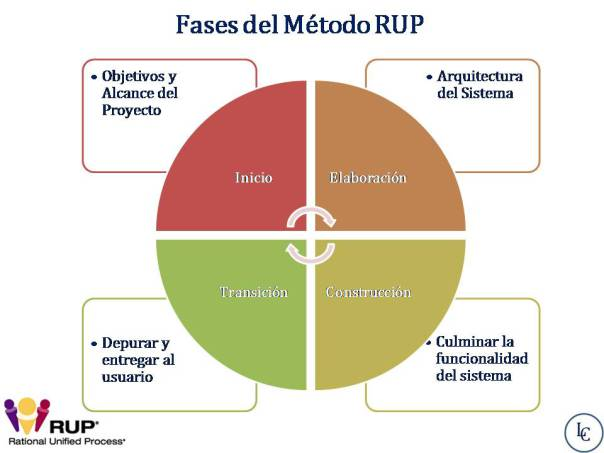
\includegraphics[width=\linewidth]{img/fases-rup.jpg}
	\endminipage\hfill
	
\end{figure}


\begin{itemize}

    \item Fase de Inicio: Esta fase tiene como propósito definir y acordar el alcance del proyecto con los patrocinadores, identificar los riesgos asociados al proyecto, proponer una visión muy general de la arquitectura de software y producir el plan de las fases y el de iteraciones posteriores.

	\item Fase de elaboración: En la fase de elaboración se seleccionan los casos de uso que permiten definir la arquitectura base del sistema y se desarrollaran en esta fase, se realiza la especificación de los casos de uso seleccionados y el primer análisis del dominio del problema, se diseña la solución preliminar.

	\item Fase de Desarrollo: El propósito de esta fase es completar la funcionalidad del sistema, para ello se deben clarificar los requisitos pendientes, administrar los cambios de acuerdo a las evaluaciones realizados por los usuarios y se realizan las mejoras para el proyecto.

	\item Fase de Transición: El propósito de esta fase es asegurar que el software esté disponible para los usuarios finales, ajustar los errores y defectos encontrados en las pruebas de aceptación, capacitar a los usuarios y proveer el soporte técnico necesario. Se debe verificar que el producto cumpla con las especificaciones entregadas por las personas involucradas en el proyecto.	

\end{itemize}
\subsection{Cuadro Comparativo}

\section{Metodología Ágil} 
\subsection{SCRUM}
\subsubsection{Ciclo de vida}
\subsection{XP}
\subsubsection{Ciclo de vida}
\subsection{}
\subsection{Cuadro Comparativo}

\section{Cuadro comparativo [Metodologías Tradicionales vs Ágiles]} 